\chapter{Implementation}

This chapter dives into what has been done for the implementation of the TCC protocol. The chapter is divided into three main sections that describe the three ways in which TCC can be implemented. These sections are divided subsequently into three subsections defining the TCC actors. Each part describes in details how it has been implemented, including programming languages and libraries used.\\
For what concerns the browser application, I developed an extension for Google Chrome. The reason behind this choice lays in the readiness with which extensions are developed. Moreover, I was already familiar with JavaScript, language in which Chrome extensions are programmed, thus I though it might have been a very good choice. I also documented on FireFox extensions, but I didn't liked the way programmers are meant to program extensions. Thus, the implementation of the two forms of extensions found hereafter are Google Chrome extensions.

\section{General TCC Implementation}
The general TCC implementation has in play a browser extension, some services implementing the TCC protocol and a server acting as transaction manager. This section describes in details how this implementation has been done.

\subsection{Google Chrome Extension}
\label{chrome-extension-general}
This Google Chrome extension implies the use of a background page. This means that while navigating, there is always a background JavaScript file executing some methods. In this case, the method being executed is the filter method which was discussed in \ref{tcc-client-side-design}. Moreover, this extension also uses a popup page. The Google Chrome API let the programmers create popup pages, which are plain HTML, that can contain any kind of information: they are capable of getting data about the currently visualized page, as well as doing HTTP requests to gather data from somewhere else. The use I made of it is the latter, in this particular case I'm gathering information from the transaction manager.\\

\subsubsection{GUI}
For what concerns the GUI, everything is stored in the popup page. At the beginning the popup asks with a form which transaction manager server the user wants to use. When a URL is provided, the GUI contacts the server through a GET request done in AJAX but returning the whole page instead of plain XML or JSON. The reason behind this choice is the use of a simple library on the transaction manager; this will be fully explained later.

\begin{figure} [ht]
\centering
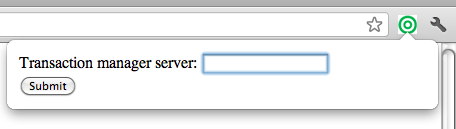
\includegraphics[scale=0.75]{images/tcc-extension-login.png}
\caption{Freedom of choice by the user for the transaction manager.}
\label{tcc-extension-login-screenshot}
\end{figure}

The server sends back the login / registration page, which is loaded in the popup and through which the user can login or register into the transaction manager service.Either of the two, the GUI loads the page containing the transaction in progress for the current logged user. If there are no transactions in progress a message informs the user of that. If instead there are transactions in progress, the user may confirm all of them clicking on a button or delete one or more by clicking on the delete button, provided for each of the transactions in progress.

\begin{figure} [ht]
\centering
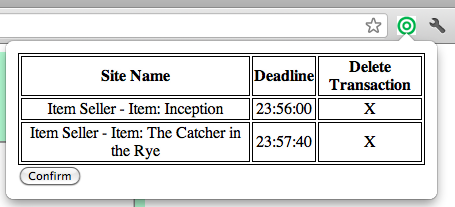
\includegraphics[scale=0.75]{images/tcc-extension-transactions-in-progress.png}
\caption{Transactions in progress for the logged user.}
\label{tcc-extension-login-screenshot}
\end{figure}

One question that may arise is: how will the GUI react if a user performs a reservation without being connected or logged in to a transaction manager? What happens is that since the server receives a reservation, it performs it and sends back the confirmation link. The extension will notice that the user has not logged in into a transaction manager so it can notify it to the user. The item will yes kept reserved, but the confirmation link will be lost. This is not a problem, in fact as the timeout expires the item will be available again.

\subsubsection{Filter}
\label{filter-general}
As mentioned in the introduction, the filter lays in the background page. Each time a request is performed and a result returned, the filter takes the result and checks if it contains a fingerprint of the TCC protocol. In that sense, the fingerprint is searched into the "Link" header of the HTTP response, and this fingerprint is {\tt /XTCC?id=}. What comes after the equal sign is the id given to that particular transaction, while what comes before the fingerprint is the URI used to reserve the item. In this way the filter finds out a confirmation link, stores it and performs a {\tt GET} request on the confirmation link through and AJAX call. This returns from the service more data regarding the transaction in JSON format. I have to specify that JSON format was asked in the header setting {\tt application/json} in the "Accept" header. The server is also programmed to return XML, if needed.\\
On the callback of this {\tt GET} request, the extension gathers the data and send it to the transaction manager through another asynchronous request (this time a {\tt PUT}), which, if the user is logged in, will store the transaction on the cloud.\\
One may think "why not sending directly all the data when sending the response of the reservation?". The reason is that the server may want to avoid sending unnecessary data (for example the name of the item reserved, the name of the website on which the item was reserved, the date in which it happened, and so on), while the client may not be interested in it and just wanting to know the remaining time to complete the transaction and the confirmation link, as well as the payload reference.\\
An interesting case to focus on is when a reservation is triggered but the service appears to be down when doing the {\tt GET} request. In that case, since {\tt GET} is an idempotent method, I used a trick: until no response is received, the filter keeps sending {\tt GET} requests doubling the time waited from one operation to the other each time one is performed. So for example the first time it will wait 1 second, then if no response is received it will wait 2 seconds, then 4 seconds, and so on. The reason is to avoid putting pressure on the service and avoiding infinite loops on {\tt GET} requests by the Google Chrome extension. This trick is called \textit{delayed request execution} and it's also used when, after receiving the additional data, the filter tries to send it to the transaction manager. If at that particular time the transaction manager is down or is experiencing major delays, the delayed request execution will delay step by step its {\tt PUT} requests (which, again, are idempotent) until the transaction manager responds.\\
Delayed request execution is used also in other contexts regarding TCC, especially in the transaction manager's work. 

\subsection{Node Service}
\label{tcc-node-service-description}
The service I implemented is a very simple dummy item seller, which sells any kind of item. It is implemented with Node.js, the server side JavaScript framework. I've chosen to work with it because Google Chrome works all in JavaScript, so I preferred to keep the same programming language all over to avoid issues like translating data models from one language to the other. Moreover, it's really simple and fast to create a server, so that I could have quickly tested my TCC implementation.\\
This services has nothing different from any other webstore. It implements MongoDB as database, and makes use of Mongoose, a library that makes easy the interaction between the server and the database. The database is used to store the items sold by the webstore and the informations about current transactions in progress. The service also makes use of Express.js, a high performance framework to simplify even more the creation of a RESTful service in Node.js.\\
When a {\tt POST} request is received to reserve an item, the service creates a new resource, accessible through a URI provided with a unique id. This URI is what is called confirmation link and it responds to {\tt GET}, {\tt DELETE} and {\tt PUT} requests. As soon as the resource is created, first it is added to the database, storing the timeout, the name of the item (or the item id) and the unique id created, and then the total amount of items of the kind of the one ordered is decreased by one.Then a timeout is setup: this timeout when expired will make the reserved item available again, thus effectively increasing the total amount of that item by one.\\
When a {\tt GET} request is received on a transaction resource, first the server checks in the database if there is a reservation with that id, then if there is, it makes up either a JSON or an XML (depending on the "Accept" header) containing all the information about the item being reserved and the reservation, then sends it back as response. If there is no reservation with that id, the server just ignores the request, since it may be the case that the reservation timed out and was removed from the database.\\
When a {\tt DELETE} request is received on a transaction resource, again the server checks in the database if that reservation still exists, and if it is the case, then in removes the database entry for that reservation and increases the total amount of the item reserved by one in the item database. This is what happens also in the case of a timeout.
When a {\tt PUT} request is received, the server checks if the reservation still exists, then if it is the case it removes the entry in the reservation database and starts the payment procedure. It is as simple as that since the total amount of items available was already decreased when the item was reserved and the server doesn't even need to remove the timeout in progress, because the timeout itself when expiring will check if the transaction is still there, and if it's not the case it means that either it has been confirmed or canceled, so no operation is performed.\\
What happens when the service goes down? Thanks to the database storing all the information about the reservation in progress, the service can set up all the timeouts again as soon as it is up and running, effectively not losing anything. If a timeout expires while the service is down, as soon as it is in the process of setting timeouts up again, it will check if the timeout expired, and if it's the case it will follow the same procedure as when a timeout expired or a {\tt DELETE} request is received.

\subsection{Node Transaction Manager}
\label{node-transaction-manager-general}
The transaction manager I implemented is also very simple. Also in this case, MongoDB was used as database, as well as Mongoose and Express.js as library and framework for the implementation.\\
The transaction manager has a page where users can login or register to the service. This page is an HTML page, so users may login either from the browser and from the Google Chrome extension. Once logged in (or registered), users may see (again either from browser or Chrome extension) the current transaction in progress.\\
As explained in \ref{chrome-extension-general}, the transaction manager has an interface to receive {\tt PUT} requests from the Google Chrome extension. When a request is received, it creates an entry in the database with all the data received (i.e. confirmation link, timeout, etc.). It also sets up a timeout, like the service, which when expired removes the transaction from the database. In this way the transaction manager is always aware of which reservation are still in progress and which are timeout (thus effectively updating the view).\\
When a {\tt GET} request is received, if the user is logged in the transaction manager shows the current transaction in progress. From this page, the user can either confirm all transactions in progress or delete one (or more). If the user decides to delete a transaction, a {\tt DELETE} requests is triggered to the transaction manager with the id of the transaction. The transaction manager first checks if the reservation is still there (since it may have timed out in the mean time), then if found, it removes it from the database and sends a {\tt DELETE} request to the confirmation link. If no response is received, it means that there is some problem with the service. In this case it makes use of the delayed request execution, which will guarantee that sooner or later the {\tt DELETE} request will reach the service. Since also {\tt DELETE} is an idempotent method, we do not have to worry if it has been received more than once at the service.\\
When a {\tt PUT} request is done for a confirmation of all the transaction in progress, the transaction manager first gathers all the transaction in progress for the user that just sent a confirmation. Then it starts sending {\tt PUT} requests on the confirmation links. Again, if one or more services are busy or down, the delayed request execution guarantees that sooner or later the {\tt PUT} request will be received by the services.\\
For what concerns timeouts, the same holds also in the transaction manager: the timeout triggers automatically the delete process triggered by a {\tt DELETE} method request. When confirming (or deleting) the timeout may be left there, since as it expires, it first checks that the transaction (for which it has been set up) is still there. If it is, delete process, if it isn't then nothing is performed.\\
One may wander what happens if the transaction manager fails and goes down. For what concerns the receiving the {\tt PUT} requests from clients, as specified in \ref{filter-general}, the delayed request execution from the Google Chrome extension will guarantee that the transaction manager will receive the reservations as soon as it gets up and running. If the failure happens before the confirmation phase, then thanks to the database persistence, the transaction manager may setup again the timeouts and has all the information about the current transactions in progress.\\
In the worst (and most interesting) case, the transaction manager may fail during the confirmation phase. What has been done in this case is the following: as soon as transaction manager gathered all the transaction in progress for the user that triggered the confirmation, it sets each reservation as "pending" in the database. When a transaction is confirmed and a response is received, the entry in the database for that transaction is removed. If the transaction manager goes down during this process, when getting up it will notice that some reservation are in "pending" state. This means that it was confirming them but something happened. In this case it will start confirming all the pending transactions again.

\section{Transaction Manager integrated in Browser Extension}
This version of the TCC protocol has the transaction manager integrated into the Google Chrome extension. For what concerns the service, I used the same service described in \ref{tcc-node-service-description} without changes. This may show how the service side of the protocol may stay invariant while we have different possibilities at the client side.

\subsection{Google Chrome Extension}
This particular version of the Google Chrome extension has the transaction manager integrated. This means that no service is needed and especially no login. The GUI is similar to what shown in figure \ref{tcc-extension-login-screenshot}, and if there are no transactions in progress, the GUI will notice it to the user.\\
Also the filter element is the same, but instead of sending a {\tt PUT} request to a transaction manager on the cloud, it stores everything in the local storage. Local storage is a form of web storage on the client side. It is accessible through JavaScript and it's a simple key/value pair storage. It is persistent, thus if there is a failure in the client side, or simply the client is shut down, the storage remains until the user wants to use it again.\\
Storing and retrieving information from the local storage works by just doing a couple of method calls, no database needed. This is a very powerful tool, because in this way the transaction manager has a very simple work. When transaction are asked (the popup of the extension is opened), it checks in the database if there are transactions in progress. If there are, it shows them. If a reservation is deleted, the transaction manager takes the confirmation link of that transaction and performs a {\tt DELETE} request, and the transaction is removed from the local storage. If instead the confirmation is triggered, the transaction manager takes all the transactions from the database and executes {\tt PUT} requests on their confirmation link.\\
For what concerns persistence in failures during confirmation phase, since the storage is a key/value pair which accepts strings, JavaScript objects are stored as plain JSON. To these object then I can add as many parameters as needed. During the confirmation phase the same "pending" state is added (as the one in \ref{node-transaction-manager-general}), and when the transaction is confirmed, it is also removed from the local storage.\\
During confirmation and deletion, as well as when asking for more information to the service, the same principle of the delayed request execution is used, so until no response is received, it will try to execute the requests in a delayed fashion.

\section{TCC used in server interaction}
The previous sections have shown how the TCC protocol can be used to control transactional interactions between a server and a client. This idea can be extended and applied to the interaction between servers with the same results: when a server needs some resources from within itself (in large applications) or from other servers, it can use the same exact protocol, having the transaction manager local to avoid network delays. The result is a server application capable of taking different resources at once when needed without the worry of gathering just some of them but not all.\\
The following subsections will introduce how the TCC idea was extended to server applications. First there will be a short introduction to S, a new programming language, on which the TCC construct is applied. Then the following two subsections will describe the TCC library and the transaction manager library created to support TCC on S.

\subsection{Introduction to S}
S is a new domain-specific programming language developed at the Universit� della Svizzera Italiana. It targets server side scripting of high-performance RESTful web services. S brings an innovative programming model, based on explicit and implicit parallelism control, which allows the service developer to specify which portion of the control-flow has to be executed in parallel. The choice of the best level of parallelism is then left to the runtime system, for each service. S compiles in Node.js, thus the executable are simple JavaScript files runnable by Node.
What has been done in the context of S is the following: since S compiles in a Node.js executable file, I took what was a simple set of operations done on a service TCC-capable (see \ref{tcc-node-service-description}) and created, through S, a server that contacts the service and reserves a couple of items. What was created in pure S was just the {\tt POST} request to the service. What I manually added later are a TCC library to support TCC transactions and a transaction manager library to support the managing of transactions in progress. The idea is to demonstrate how, applying a small change to the compiler, we can compile S and generate code that supports TCC just by adding the following two libraries.

\subsection{TCC Library}
This library is made of a constructor, an init method and a reserve method. The constructor returns a new object of the type TCC, which is the type defined by the library. The init method takes a transaction manager, a URI and a scheduler. The transaction manager is needed when a confirmation link is retrieved. The idea is that once this TCC object has filtered a confirmation link, it directly stores it into the transaction manager. The URI is the address to which we perform a {\tt POST} request to reserve items on the service. The scheduler is a construct from S which is used to schedule subsequent actions when this one is complete (e.g. after this execution the scheduler will emit an event that will trigger the next execution).\\
The reserve method takes as parameter a event, which will be the input of the emit method of the scheduler, which will be called when the execution of the reservation is over. The reservation is done in a similar fashion to what the client in the Google Chrome extension does. First, it creates a {\tt POST} request to the URI provided in the constructor. Then when the result is received, it is filtered to gather the confirmation link. With this, a hidden method is called to gather more information about the transaction (the {\tt GET} request). I call this method "hidden" because it is not visible to the outside of the library. After the result of the {\tt GET} request are gathered and ordered, they are set into the transaction manager. Finally, the scheduler emits the event passed as parameter.\\
If some error occurs during the reservation process, the scheduler emits the event and an error is logged. For what concerns failure resistance in this case, still nothing has been done. One idea could be to notify in some way the transaction manager object with the link of the resource that has not been able to contact. In this way we may set up an ideal system in which if more than an input number of reservation fails, the transaction manager does not confirm the transactions at the end.

\subsection{Transaction Manager Library}
The transaction manager library is made of a constructor, an init function, a function to store links, a function to delete transactions and one to confirm them all. The constructor and the init function have no parameter. The first one simply returns an object of the type TransactionManager. The second one creates the array of confirmation links. The function to store link takes as parameter an object containing the confirmation link as well as other informations about the transaction in progress, the link is taken and added to the previously created array, then a timeout is created which, when fired, removes the object from the array. In this way when confirming, if one timed out, it will not be confirmed.\\
The function to delete transactions takes a confirmation link and performs a {\tt DELETE} request on it in delayed request execution fashion. The same trick is used when performing a confirmation through the confirm method. It takes all the links stored in the array and performs a {\tt PUT} request on them with the delayed request execution. If there is some timeout during confirmation it is kept into account. \\
One may notice that there is no persistence in all of this. Persistence in this case can be made possible by simply adding a database storage to the library, but the purpose of this study was to demonstrate how easily one can extend his own server with the TCC protocol. Many implementation are possible, the reader is invited to develop and explore his own.
